\section{MODULE DESIGN}
\subsection{DATA PREPROCESSING}
JPEG uses a lossy image compression. Each re-encoding process (new saving) performed on the image leads to further loss of quality. The JPEG algorithm is based on a 8x8 pixel grid. Each 8x8 square grid is thereby treated and compressed separately. If the image is untouched, then all these 8x8 squares will show the same error level potential.  
\subsubsection{Algorithm:} 
\begin{enumerate}
    \item The image is resaved with 95\%(or 90\%)JPEG quality.
    \item Compare each(8*8) blocks of corresponding original and new resaved image. 
\item If image is unmodified, then all 8 x8 squares should have similar error potentials.
\item Else modified areas will appear with a higher potential error level.
\end{enumerate}

INPUT \ \ \ \ : Tampered image

OUTPUT : The output of ELA is image with higher error potential.

\subsection{TRAINING THE CNN}
\begin{figure}[htp]
\centering
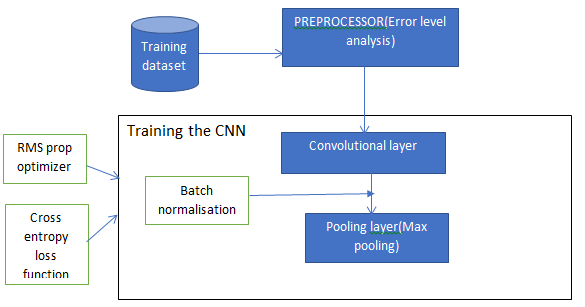
\includegraphics[scale=0.5,width=17cm]{Figures/cnn.PNG}
\caption{Training the model}
\label{fig:universe}
\end{figure}
The training process of a CNN is done through an iterative algorithm that alternates between feedforward  and back propagation passes of the data. The weights of the convolutional filters and fully-connected layers are updated at each iteration of the backpropagation passes. CNN is capable of learning classification features directly from the data. The ReLU activation function is applied to each value in the feature maps of every convolutional layer. The convolutional layers are followed by the max pooling layers. We use a batch normalization layer after each regular convolutional layer. However, the prediction error convolutional filters outputs are directly convolved with the next convolutional layer without using the batch normalization layer. We consider the RMSProp optimizer  to train our model. This module is proposed to extract features related to the traces left by different editing operations, and which are utilized to check the authenticity of images. 

INPUT \ \ \ \ : The pre-processed images.

OUTPUT : The trained classifier to detect the tampered images.

\subsubsection{Algorithm:}
1. Initialize w_k 's\  using \ randomly\  drawn\  weights.
    
2. Assign i=1

3. While  i \leq  maximum\_iteration \ do

4. Feedforward  pass.

5. Update filter weights  and backpropagate errors.

6. Set w_k(0, 0)^(^1^) = 0  for \ all \ K \ filters

7. Normalize w_k^(^1^)  ’s \ such \ that \  \Sigma_l_,_m_ \neq _0 w_k^(^1^)   (l, m) = 1

8. Set w_k(0, 0)^(^1^) = - 1  \ for \ all \  K \ filters

9. i = i + 1

10. If training accuracy converges then

11. exit

12. end
\newpage
\subsubsection{RMSPROP OPTIMISER }
The RMSprop optimizer is similar to the gradient descent algorithm with momentum. The RMSprop optimizer restricts the oscillations in the vertical direction. Therefore, we can increase our learning rate and our algorithm could take larger steps in the horizontal direction converging faster. 

              vdw =\beta. vdw  + (1- \beta).dw2  
                 
                     where  \beta \ is \ a \ momentum \ in \ learning \ rate 
              
              vdb  = \beta. vdw  + (1- \beta).db2
              
              W = W -\alpha dw/(\sqrt(v\_db )+∈)      
                     
                     where W are weights to be updated during the back propagation and  \alpha \ is \ a \ value \  always \textless 1.      
               
              b = b - \alpha dw/(\sqrt(v\_db )+\epsilon)     
              
                     where b is the calculated gradient of the system while learning and \epsilon \  is\ a \ small \ value \  added \ to \ prevent \ gradient \ from \ blowing \ up.

\subsubsection{CROSS ENTROPY LOSS FUNCTION}
Cross Entropy is commonly-used in binary classification (labels are assumed to take values 0 or 1) as a loss function (For multi-classification, use Multiclass Cross Entropy), which is computed by  

       L=-1/n \Sigma_(i_=_1)^n [\ (\ y^(^i^)  log(\ \^y^i)\ +(\ 1-y^i)log(\ 1-\^y^i) ]\

Where L is a loss calculated which is the difference between the actual and the predicted output. 
Cross entropy measures the divergence between two probability distribution, if the cross entropy is large, which means that the difference between two distribution is large, while if the cross entropy is small, which means that two distribution is similar to each other. When the difference between predicted value and actual value is large, the learning speed, i.e., convergence speed, is fast, otherwise, the difference is small, the learning speed is small. Cross entropy cost function has the advantages of fast convergence and is more likely to reach the global optimization. 

\subsection{CLASSIFICATION BLOCK}
\begin{figure}[htp]
\centering
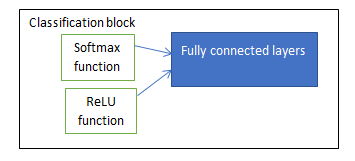
\includegraphics[scale=0.5,width=10cm]{Figures/soft.PNG}
\caption{Classification}
\label{fig:universe}
\end{figure}
This first layer of the classification block contains about 256 nodes and accepts input as vectors. This layer uses ReLU activation function where negative values will not be considered significant hence makes it more efficient. To give the accurate result the last layer in the classification block of the neural network uses the softmax activation function which gives the highest activation level. The CNN model extracts the feature and classifies the pre-processed forged image to detect whether the given image is spiced or not.

\subsection{COPY MOVE TYPE DETECTION}
A copy move attack is commonly used to conceal parts of an image or to remove unwanted portions in an image. A portion from the picture is copied and pasted over any unwanted portion in the same image.
This block is where the image that is not detected to be spliced is checked for copy move forgery using the following steps:
\begin{enumerate}
    \item Blur image for eliminating image details.
    
\item Convert image to degraded palette.

\item Decompose the image into small NxN pixel blocks.

\item Alphabetically order these blocks by their pixel values.

\item Extract only these adjacent blocks which have small absolute color difference.

\item Cluster these blocks into clusters by intersection area among blocks.

\item Extract only these clusters which are bigger than block size.

\item Extract only these clusters which have similar cluster, by using some sort of similarity function (in this case Hausdorff distance between clusters).

\item Draw discovered similar clusters on image.

\end{enumerate}


\section{COMPLEXITY ANALYSIS}
\subsection{COMPLEXITY OF THE PROJECT}
\begin{itemize}
    \item  The complexity of the project lies in determining the passive type of forgery the image has undergone  rather than just determining if the image is only forged or not. The neural network is used to detect the spliced images.
    \item The accuracy of the neural network also affects the efficiency of the output. Hence efficient loss function and optimiser with the appropriate parameters needs to be chosen. 
    \item Certain additional hints need to be added to the images in order to efficiently detect the tampered regions in the images. Error Level Analysis is used for this purpose. This analysis is made to all images irrespective of their formats and error potential.  
    \item Determining the identical regions in a copy move image is done by the extraction of similar properties between those regions for which efficient similarity functions has to be used. 
    \item The identification of copy move image is done without any comparison with the original image but rather the input image itself which makes it a tedious task to implement.
\end{itemize}